\documentclass[11pt]{article}
\usepackage[a4paper,margin=2.5cm]{geometry}
\usepackage[utf8]{inputenc}
\usepackage[T1]{fontenc}
\usepackage{lmodern}
\usepackage{amsmath,amssymb}
\usepackage{booktabs}
\usepackage{graphicx}
\usepackage{siunitx}
\usepackage[numbers,sort&compress]{natbib}
\usepackage{xcolor}
\usepackage[colorlinks=true,linkcolor=blue!50!black,citecolor=blue!50!black,urlcolor=blue!50!black]{hyperref}
\usepackage{caption}
\captionsetup{font=small,labelfont=bf}
\graphicspath{{figures/}}

% Generated by code/paper/make_paper_figures.py; do not edit.
\newcommand{\NdoeCases}{384}
\newcommand{\NtrainCases}{288}
\newcommand{\NevalCases}{96}
\newcommand{\NholdoutCases}{48}
\newcommand{\NboundaryCases}{24}
\newcommand{\NpressureCases}{24}
\newcommand{\RtwoCvMlp}{0.862}
\newcommand{\RtwoCvRidge}{0.796}
\newcommand{\RtwoEvalMlp}{0.778}
\newcommand{\RtwoEvalRidge}{0.727}
\newcommand{\DeltaRtwoCv}{0.066}
\newcommand{\Cmin}{1.00}
\newcommand{\Cmax}{4.51}
\newcommand{\Cmedian}{1.42}
\newcommand{\NgaDesigns}{17}
\newcommand{\NgaConsMax}{4}
\newcommand{\NgaConsPninetyfive}{17}
\newcommand{\NgaMaxAboveOne}{5}
\newcommand{\NdomeCritical}{198}
\newcommand{\NdomeCriticalHoop}{179}
\newcommand{\NcylCritical}{103}
\newcommand{\NjunctionCritical}{56}
\newcommand{\NbossCritical}{27}
\newcommand{\NdoeInconsistent}{202}
\newcommand{\NdoeConsistent}{182}
\newcommand{\MetricsTableCv}{$-3.910 \pm 0.207$ & $0.791 \pm 0.047$ & $0.796 \pm 0.046$ & $0.862 \pm 0.029$}
\newcommand{\MetricsTableEval}{$-4.015$ & $0.717$ & $0.727$ & $0.778$}
\newcommand{\MetricsTableHoldout}{$-5.900$ & $0.770$ & $0.787$ & $0.789$}
\newcommand{\MetricsTableBoundary}{$-2.270$ & $0.647$ & $0.672$ & $0.800$}
\newcommand{\MetricsTablePressure}{$-4.016$ & $0.726$ & $0.703$ & $0.714$}
\newcommand{\HoopZeroBefore}{0.86}
\newcommand{\HoopZeroAfter}{1.16}
\newcommand{\MeshPeakLow}{0.85}
\newcommand{\MeshPeakHigh}{1.11}
\newcommand{\NpeakAtPole}{205}
\newcommand{\CninetyfiveMedian}{0.99}
\newcommand{\CninetyfiveMin}{0.94}
\newcommand{\CninetyfiveMax}{1.40}
\newcommand{\NCninetyfiveWithinTen}{369}
\newcommand{\TargetRowBaselineMax}{$0.79$ & $0.72$ & $0.80$ & $0.73$ & $0.86$ & $0.78$}
\newcommand{\TargetRowBaselinePninetyfive}{$0.20$ & $0.26$ & $0.17$ & $0.27$ & $0.27$ & $0.48$}
\newcommand{\RtwoCvMlpPninetyfive}{0.27}
\newcommand{\RtwoEvalMlpPninetyfive}{0.48}
\newcommand{\TargetRowStrictMax}{$0.53$ & $0.17$ & $0.51$ & $0.21$ & $-0.10$ & $-1.25$}
\newcommand{\TargetRowStrictPninetyfive}{$0.65$ & $0.16$ & $0.63$ & $0.48$ & $0.20$ & $-0.33$}
\newcommand{\NstrictTrain}{138}
\newcommand{\NstrictEval}{44}
\newcommand{\RtwoEvalRidgeStrictPninetyfive}{0.48}
\newcommand{\CstrictMedian}{2.74}
\newcommand{\CstrictMax}{6.87}
\newcommand{\CstrictNinetyfiveMedian}{1.07}
\newcommand{\NstrictDome}{177}
\newcommand{\MeshBasePninetyfiveFortyEight}{0.4}
\newcommand{\MeshBasePninetyfiveTwentyFour}{3.7}
\newcommand{\MeshStrictPninetyfiveFortyEight}{18}
\newcommand{\MeshStrictMaxLow}{0.51}
\newcommand{\MeshStrictMaxHigh}{2.64}
\newcommand{\MeshTimeSixtyFour}{11}
\providecommand{\MeshPeakLow}{?}
\providecommand{\MeshPeakHigh}{?}


\newcommand{\FI}{\mathrm{FI}}

\title{Learning a dome correction for Type~IV hydrogen vessel sizing from 384 shell simulations, and an audit of the high-fidelity target}
\author{Cl\'ement Dumeril\thanks{University of California, Berkeley (MEng). The work started as an Arts et M\'etiers group assignment in May--June 2026; all modelling, code and analysis reported here are the author's. Code and data: \url{https://github.com/clementdumeril/copv-type4-multifidelity}.}}
\date{October 2026}

\begin{document}
\maketitle

\begin{abstract}
Genetic-algorithm layup optimizers for Type~IV hydrogen vessels rely on sizing models that run in about a millisecond and ignore the dome. I built a CalculiX shell model of the whole vessel with geodesic winding, solved \NdoeCases{} designs of an 11\,L vessel, and trained a multilayer perceptron (MLP) to predict the ratio $C$ between the maximum fiber failure index of the shell model and that of a thick-cylinder model. On this dataset the MLP reaches a cross-validated $R^2$ of \RtwoCvMlp{} on $\log C$ (ridge regression: \RtwoCvRidge{}) and \RtwoEvalMlp{} on \NevalCases{} held-out designs. Inside the optimizer, the corrected index stays above the 95th percentile of the shell-model index for all \NgaDesigns{} optimized designs, but above its maximum for only \NgaConsMax{}. An audit of the target explains this gap. The maximum sits at the polar opening in \NpeakAtPole{} designs and is not mesh-converged. It depends on a coverage floor that keeps part of every ply below its turnaround radius, and \NdoeInconsistent{} designs pair a helical angle and a boss radius that geodesic winding cannot connect. Computed on the mesh-converged 95th percentile, $C$ is within 10\,\% of 1 for \NCninetyfiveWithinTen{} of \NdoeCases{} designs, and on the geometrically consistent designs no corrector generalizes. The learned correction is therefore a correction of a numerical peak, useful as a conservative margin, not evidence of a physical dome effect.
\end{abstract}

\section{Introduction}

Type~IV vessels store hydrogen at \SIrange{35}{70}{MPa} in a polymer liner overwrapped with filament-wound carbon/epoxy. Burst is usually governed by fiber failure, and the dome, the dome--cylinder junction and the boss region are where geometry, winding angle and thickness change fastest \cite{Leh2015,Hu2021,Jois2021}. Layup optimization by genetic algorithm (GA) evaluates tens of thousands of stacks, so the structural model inside the loop has to be cheap. The optimizer studied here uses an analytical thick-cylinder model that is accurate for the cylindrical section and blind to the domes.

The initial question was whether a correction learned from a dome-resolved finite-element model can make such an optimizer aware of the dome without slowing it down or modifying its code. Answering it required a closer look at the finite-element target itself, and that look changed the answer.

Contributions:
\begin{itemize}
\item A pipeline that couples a CalculiX composite-shell model, a \NdoeCases{}-case design of experiments (DOE), a correction model compared with linear baselines on two extrapolation regimes, and the GA, with every optimized design re-solved in CalculiX.
\item An audit of the high-fidelity target: location of the peak, mesh study up to $64\times64$ elements, ablation of the ply-coverage law near the pole, and a check of the geometric consistency of the DOE.
\item A re-analysis with the mesh-converged quantity and the consistent designs, and a comparison of the shell model with six published burst tests, one of which it does not reproduce.
\end{itemize}

\section{Related work}

Multi-fidelity methods combine cheap and expensive models to reduce the cost of optimization and uncertainty propagation \cite{Peherstorfer2018}. Discrepancy models go back to the Bayesian calibration framework of Kennedy and O'Hagan \cite{KennedyOHagan2001}; neural networks have been used to learn the map from low- to high-fidelity outputs \cite{MengKarniadakis2020}. The present work is a simple instance, a multiplicative correction learned on scalar outputs with the low-fidelity code left unchanged. Like any such method, it is only as reliable as the high-fidelity data, which is the point examined here.

Progressive-failure finite-element models of Type~IV vessels reproduce burst pressures within a few percent when the layup, dome thickness and damage law are known \cite{Leh2015,Hu2021,Jin2022,Agne2025}. Dome thickness and fiber angle follow from the winding: geodesic paths obey Clairaut's relation and tows accumulate near the turnaround radius \cite{Wang2022}; the dome contour changes the stress state near the junction \cite{Jois2021}. Lamina failure is assessed with interactive or mode-based criteria \cite{TsaiWu1971,Hashin1980,Puck1998}. The fast model uses Lekhnitskii's solution for an anisotropic layered cylinder \cite{Lekhnitskii1963}. Open burst-test data with full layup documentation are rare; the DLR dataset of L\"uders et al.\ \cite{Lueders2025} is one exception.

\section{Models}

\subsection{Fast analytical model}
The fast model belongs to an existing GA code that the author did not write. Each ply of the cylindrical wall is a cylindrically orthotropic layer; continuity of radial displacement and radial stress at every interface gives a linear system for the stresses under internal pressure \cite{Lekhnitskii1963}. Ply stresses are rotated into the material frame and checked with the Hashin, Tsai--Wu and Puck criteria. One evaluation takes under a millisecond. The model has no dome, no boss and no change of winding angle; in all \NdoeCases{} designs it places the critical point in the cylinder.

\subsection{Dome-resolved shell model}
The reference model covers the cylinder, both domes and the polar openings with eight-node reduced-integration shells (S8R) in CalculiX 2.23 \cite{Dhondt2024}. The meridian profile is hemispherical, isotensoid-like or a variable contour. Each element carries its own composite section with local ply angles and thicknesses. Helical and transition plies follow the geodesic law $\sin\alpha(r) = r_t/r$, where $r_t = R\sin\alpha_0$ is the turnaround radius of a ply wound at $\alpha_0$ on the cylinder of radius $R$; hoop plies keep their nominal angle (86.5 to 89.5\textdegree). Near its turnaround radius a ply's thickness is multiplied by a logistic coverage weight, which tends to a floor $\varepsilon$ below that radius ($\varepsilon$ is sampled between 0.20 and 0.35). The liner is not modelled. One boss is fixed axially and the other slides, so the vessel elongates without an artificial axial clamp. The internal pressure is applied with \texttt{*DLOAD}, the axial force on the polar openings with \texttt{*CLOAD}, and the analysis is linear static. Table~\ref{tab:material} gives the lamina properties.

\begin{table}[t]
\centering
\caption{Lamina properties of the carbon/epoxy used in the DOE (\texttt{code/config/material\_database.json}).}
\label{tab:material}
\begin{tabular}{cccccccccc}
\toprule
$E_1$ & $E_2=E_3$ & $G_{12}$ & $\nu_{12}$ & $\nu_{23}$ & $X_T$ & $X_C$ & $Y_T$ & $Y_C$ & $S_{12}$ \\
\multicolumn{3}{c}{[GPa]} & & & \multicolumn{5}{c}{[MPa]} \\
\midrule
151 & 9 & 5 & 0.30 & 0.42 & 2000 & 1500 & 50 & 200 & 80 \\
\bottomrule
\end{tabular}
\end{table}

\subsection{Fiber failure index and correction factor}
Shell stresses at the section points are assigned to plies from their radial position, averaged per ply and per element, and rotated into the fiber frame. The fiber index of a ply is $|\sigma_{11}|/X_T$ in tension and $|\sigma_{11}|/X_C$ in compression. The vessel index $\FI$ is the maximum over all (element, ply) pairs; the 95th and 99th percentiles over the same pairs are also recorded. I first used the combined Hashin/Tsai--Wu/Puck index, but its matrix and shear terms reach values in the hundreds near the polar opening at service pressure. The correction factor is
\begin{equation}
C = \FI^{\mathrm{FE}} / \FI^{\mathrm{fast}},
\end{equation}
which lies between \Cmin{} and \Cmax{} over the DOE (median \Cmedian{}).

\section{Design of experiments, correction model and optimizer coupling}

\paragraph{DOE.} All designs have an internal volume of 11\,L; the cylinder length follows from the radius and dome shape. Table~\ref{tab:doe} lists the sampled parameters. Case roles are fixed before training: \NtrainCases{} training designs, \NholdoutCases{} in-distribution holdouts, \NboundaryCases{} designs at the edge of the geometric ranges and \NpressureCases{} at untrained pressures. Every design was solved at $24\times24$ elements (six elements along each dome meridian).

\begin{table}[t]
\centering
\caption{Sampled parameters of the 11\,L DOE (\texttt{data/doe\_11l\_single\_boss\_cases.json}).}
\label{tab:doe}
\begin{tabular}{ll}
\toprule
Parameter & Range \\
\midrule
Inner radius $R$ & 76--96\,mm (cylinder 257--550\,mm) \\
Boss radius & 21.5--34.1\,mm \\
Dome shape & hemispherical, isotensoid-like, variable contour \\
Helical angle on the cylinder & 12--26\textdegree \\
Helical / transition / hoop pairs & 4--5 / 1--2 / 2--3 \\
Total thickness & 10.5--26.1\,mm \\
Coverage floor $\varepsilon$ & 0.20--0.35 \\
Pressure & 70\,MPa; 52.5 and 87.5\,MPa for the pressure split \\
\bottomrule
\end{tabular}
\end{table}

\paragraph{Correction models.} The target is $\log C$. Inputs are 17 design and fast-model quantities, six derived ratios ($pR/t$, boss-to-radius ratio, length-to-radius ratio, hoop and transition pair fractions, helical--hoop angle gap) and the one-hot dome shape, standardized with training-set statistics. Four models are compared: a constant, ordinary least squares (OLS), ridge regression ($\alpha=10$) and an MLP with hidden layers of 24 and 12 tanh units, written in NumPy with hand-coded backpropagation and trained full-batch with Adam \cite{KingmaBa2014} (learning rate 0.002, L2 penalty $4\times10^{-4}$, 6000 epochs, fixed seed). Cross-validation uses 8 folds repeated 4 times, on the training designs only. No design appears twice and none is shared between training and evaluation.

\paragraph{Optimizer coupling.} The GA maximizes the ratio of inner to outer radius (thinnest wall), keeps the proportions of ply angles near targets, and penalizes designs whose failure index exceeds 1 at the 87\,MPa design burst pressure. The coupling replaces the fast fiber index by $\FI^{\mathrm{fast}}\,\hat C(\mathbf{x})\,\exp(m_{95})$, where $\hat C$ is the MLP prediction and $m_{95}$ the 95th percentile of its cross-validation residuals on $\log C$.

\section{Results on the original dataset}

Table~\ref{tab:metrics} gives the scores on $\log C$ and Fig.~\ref{fig:scatter} the held-out predictions. The MLP is ahead of ridge regression by \DeltaRtwoCv{} in cross-validated $R^2$, and clearly ahead only at the edge of the geometric domain; at untrained pressures OLS does slightly better. Re-running the validation script on the committed dataset reproduces every metric exactly.

\begin{table}[t]
\centering
\caption{$R^2$ on $\log C$ for the original target (\texttt{data/extended\_statistical\_metrics.json}). CV: mean $\pm$ standard deviation over 4 repeats of 8 folds on the training designs.}
\label{tab:metrics}
\begin{tabular}{lcccc}
\toprule
 & Constant & OLS & Ridge & MLP \\
\midrule
CV, \NtrainCases{} training designs & \MetricsTableCv \\
Held-out, all \NevalCases{} & \MetricsTableEval \\
\quad in-distribution (\NholdoutCases{}) & \MetricsTableHoldout \\
\quad geometric boundary (\NboundaryCases{}) & \MetricsTableBoundary \\
\quad untrained pressure (\NpressureCases{}) & \MetricsTablePressure \\
\bottomrule
\end{tabular}
\end{table}

\begin{figure}[t]
\centering
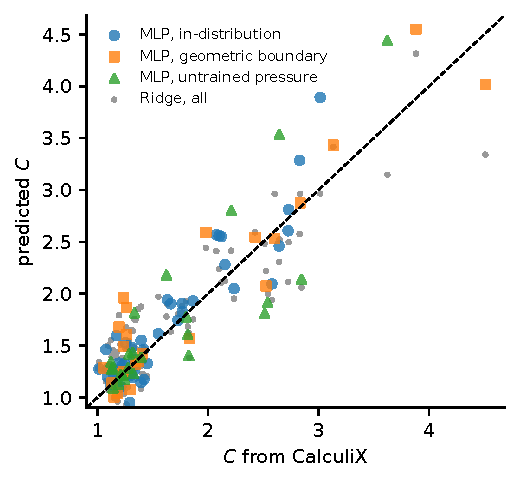
\includegraphics[width=0.55\linewidth]{fig_scatter.pdf}
\caption{Predicted against CalculiX correction factor on the \NevalCases{} held-out designs (\texttt{data/extended\_statistical\_eval\_predictions.csv}).}
\label{fig:scatter}
\end{figure}

The fast model always reports the cylinder as critical; the shell model reports a dome in \NdomeCritical{} designs, the cylinder in \NcylCritical{}, the junction in \NjunctionCritical{} and the boss edge in \NbossCritical{} (Fig.~\ref{fig:zones}). The dome peak is always on the side of the axially fixed boss.

\begin{figure}[t]
\centering
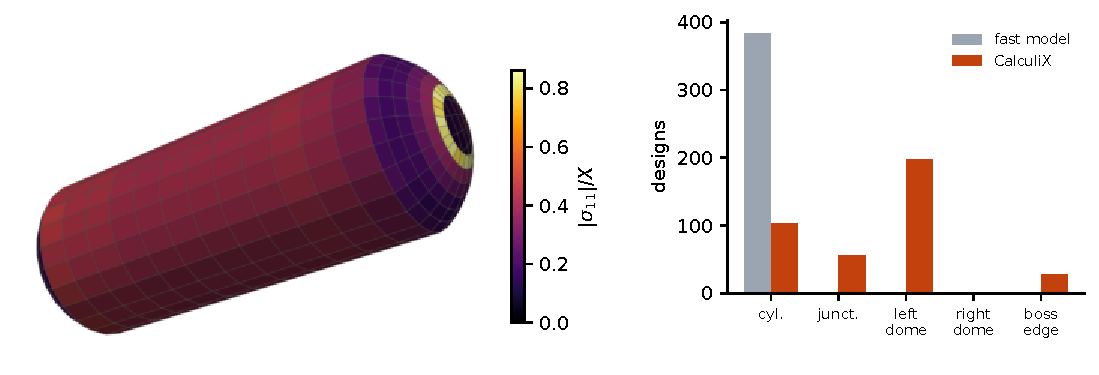
\includegraphics[width=\linewidth]{fig_field_zones.pdf}
\caption{Left: fiber index of design \texttt{11l\_0122} at 70\,MPa, worst ply per element. Right: zone of the maximum over the \NdoeCases{} designs for both models.}
\label{fig:zones}
\end{figure}

Ten GA runs with different seeds gave \NgaDesigns{} distinct designs, all with 12 plies and a 15.22\,mm wall, each re-solved in CalculiX at 87\,MPa (Fig.~\ref{fig:ga}). Without correction, the fast index is below the CalculiX 95th percentile for all of them. With the correction, it is above the 95th percentile for \NgaConsPninetyfive{} of \NgaDesigns{} and above the maximum for \NgaConsMax{}; \NgaMaxAboveOne{} designs have a CalculiX maximum above 1.

\begin{figure}[t]
\centering
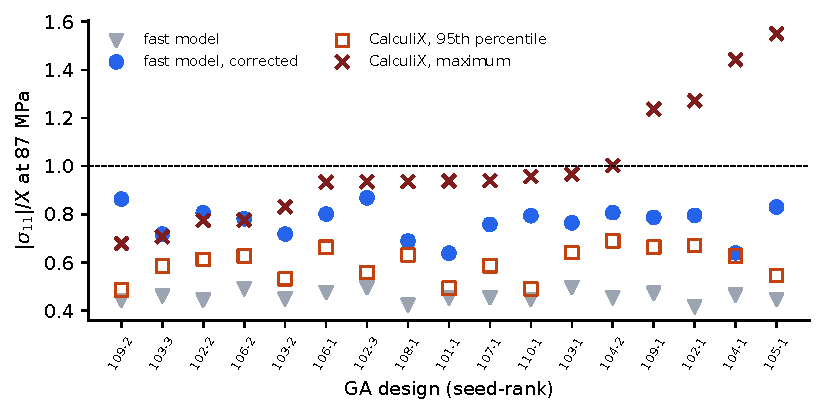
\includegraphics[width=0.85\linewidth]{fig_ga.pdf}
\caption{Fiber index of the \NgaDesigns{} GA designs at 87\,MPa (\texttt{data/ga\_statistical\_validation.csv}).}
\label{fig:ga}
\end{figure}

\section{Audit of the high-fidelity target}

\subsection{Where the maximum is}
In \NpeakAtPole{} of the \NdoeCases{} designs the maximum lies within 1.25 boss radii of the axis, that is in the ring of elements at the polar opening (\texttt{data/baseline\_fiber\_peak\_location.csv}). In \NdomeCriticalHoop{} of the \NdomeCritical{} dome-critical designs it is in a hoop ply, a ply that real winding does not place in the dome.

\subsection{Mesh study}
Four designs were re-solved at 16, 24, 32, 48 and 64 elements per direction: three dome-critical designs close to the median $C$, one per dome shape, and design \texttt{11l\_0007}, whose maximum is in the cylinder at $24\times24$ (Fig.~\ref{fig:mesh}, \texttt{data/paper\_mesh\_study.csv}; no stress sampling was applied). With the DOE coverage law (top row), the 95th percentile changes by at most \MeshBasePninetyfiveFortyEight\,\% between 48 and 64 and by at most \MeshBasePninetyfiveTwentyFour\,\% between 24 and 64: it is converged at the DOE mesh. The maximum and the 99th percentile are not. They vary non-monotonically, the critical ply changes with the mesh, and for \texttt{11l\_0007} the critical zone moves from the cylinder to the dome above $24\times24$. For design \texttt{11l\_0122} the maximum goes from \MeshPeakLow{} to \MeshPeakHigh{}.

\begin{figure}[t]
\centering
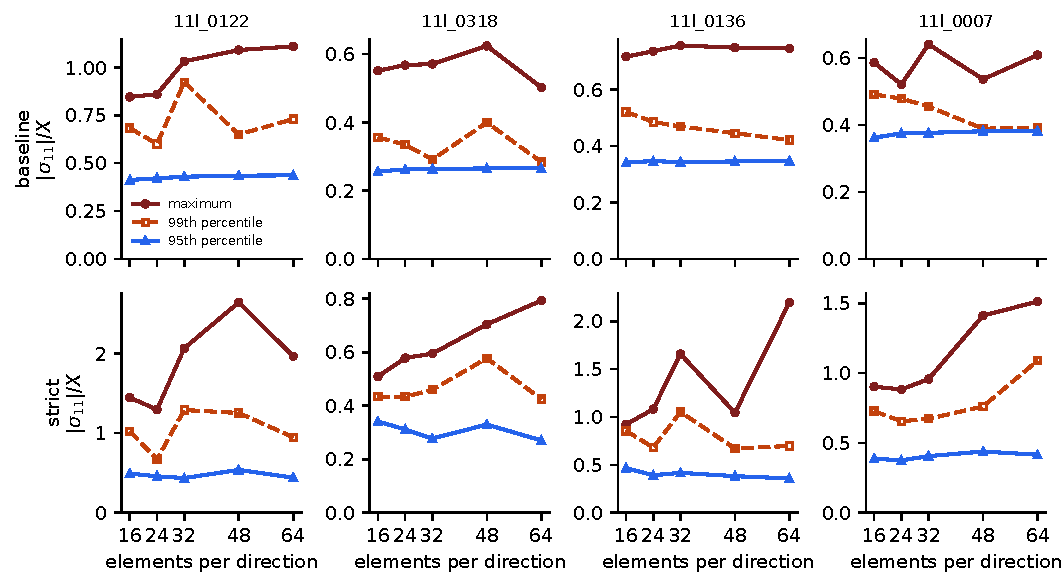
\includegraphics[width=\linewidth]{fig_mesh.pdf}
\caption{Fiber index against mesh density for four designs, with the DOE coverage law (top) and with plies stopped at their turnaround radius (bottom).}
\label{fig:mesh}
\end{figure}

\subsection{Coverage law and geometric consistency}
Removing hoop coverage from the dome does not lower the peak of design \texttt{11l\_0122}: it rises from \HoopZeroBefore{} to \HoopZeroAfter{} and moves to a transition ply at the same radius. The mechanism is general. Below its turnaround radius, a ply's geodesic angle tends to 90\textdegree, so any ply kept there by the coverage floor is nearly circumferential and carries the hoop strain of the pole, whatever its thickness.

The coverage floor also hides an inconsistency of the DOE. In \NdoeInconsistent{} of the \NdoeCases{} designs the helical turnaround radius $R\sin\alpha_0$ is larger than the boss radius, so no geodesic ply can reach the polar opening, and the floor is what covers the pole.

I re-solved the \NdoeConsistent{} consistent designs with every ply stopped at its own turnaround radius (``strict''; weights below 5\,\% are dropped). The maximum increases (median $C$ \CstrictMedian{}, up to \CstrictMax{}) and the peak stays in a dome in \NstrictDome{} designs, now mostly in transition and helical plies. This variant is not mesh-converged either (Fig.~\ref{fig:mesh}, bottom): the maximum varies between \MeshStrictMaxLow{} and \MeshStrictMaxHigh{} without trend, and even the 95th percentile moves by up to \MeshStrictPninetyfiveFortyEight\,\% between 48 and 64. Dropping plies creates thickness steps that the coverage floor had smoothed out.

\subsection{Learning other targets}
Table~\ref{tab:targets} and Fig.~\ref{fig:targets} repeat the learning protocol on three other targets. On the mesh-converged 95th percentile of the original model, $C$ has a median of \CninetyfiveMedian{} (range \CninetyfiveMin{}--\CninetyfiveMax{}) and is within 10\,\% of 1 for \NCninetyfiveWithinTen{} of \NdoeCases{} designs: away from the polar opening, the fast cylinder model and the shell model agree. Little is left to learn (MLP: \RtwoCvMlpPninetyfive{} in CV, \RtwoEvalMlpPninetyfive{} held out). On the \NdoeConsistent{} consistent designs (\NstrictTrain{} for training, \NstrictEval{} held out), none of the models generalizes; the best held-out score is \RtwoEvalRidgeStrictPninetyfive{} for ridge regression on the 95th percentile, and the MLP overfits.

\begin{table}[t]
\centering
\caption{$R^2$ on $\log C$ for four targets, same protocol (CV / held-out). Files: \texttt{data/extended\_statistical\_metrics*.json}.}
\label{tab:targets}
\small
\begin{tabular}{lcccccc}
\toprule
 & \multicolumn{2}{c}{OLS} & \multicolumn{2}{c}{Ridge} & \multicolumn{2}{c}{MLP} \\
Target & CV & held-out & CV & held-out & CV & held-out \\
\midrule
Maximum, DOE coverage (original) & \TargetRowBaselineMax \\
95th percentile, DOE coverage & \TargetRowBaselinePninetyfive \\
Maximum, strict (\NdoeConsistent{} designs) & \TargetRowStrictMax \\
95th percentile, strict (\NdoeConsistent{} designs) & \TargetRowStrictPninetyfive \\
\bottomrule
\end{tabular}
\end{table}

\begin{figure}[t]
\centering
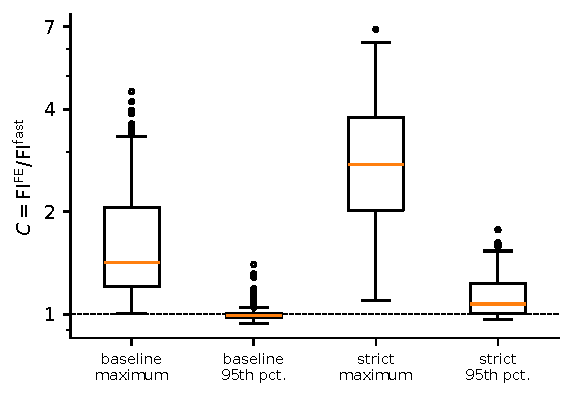
\includegraphics[width=0.6\linewidth]{fig_targets.pdf}
\caption{Distribution of the correction factor for the four targets (log scale).}
\label{fig:targets}
\end{figure}

\section{Comparison with published burst tests}
The shell model and fiber index were applied to six published vessels from four studies (Table~\ref{tab:bench}); geometry and layup were rebuilt from each paper, partly from figures. The model is conservative by 4 to 22\,\% on five of them. For Hu et al.\ the pressure matches but the location does not: the first failed ply is a cylinder hoop ply in the model and in the dome in the paper. The DLR vessel is not reproduced even with the published layup book; a 22.2\textdegree{} helical layer becomes critical near its turnaround radius, the region that the audit identifies as unreliable.

\begin{table}[t]
\centering
\caption{Shell model against published burst tests. Ranges span the maximum, 95th and 99th percentile of the fiber index; for Jin et al.\ the 99th percentile at $32\times32$ is given.}
\label{tab:bench}
\small
\begin{tabular}{llrrr}
\toprule
Source & Vessel & Measured [MPa] & Model [MPa] & Gap \\
\midrule
Hu et al.\ 2021 \cite{Hu2021} & H$_2$, first fiber damage & 161.0 & 148.7 & $-7.6\,\%$ \\
Agne et al.\ 2025 \cite{Agne2025} & GFRP & 29.39 & 25.4--27.7 & $-6$ to $-14\,\%$ \\
Agne et al.\ 2025 \cite{Agne2025} & CFRP & 27.04 & 25.7--25.9 & $-4$ to $-5\,\%$ \\
Jin et al.\ 2022 \cite{Jin2022} & EX-A & 65.20 & 58.6 & $-10\,\%$ \\
Jin et al.\ 2022 \cite{Jin2022} & EX-B & 65.17 & 50.8 & $-22\,\%$ \\
L\"uders et al.\ 2025 \cite{Lueders2025} & SN03, layup book & 25.37 & 6.5 & $-74\,\%$ \\
\bottomrule
\end{tabular}
\end{table}

\section{Discussion and limitations}
\paragraph{What holds.} The pipeline works end to end and is reproducible. Away from the polar opening, the fast cylinder model and the shell model agree to within 10\,\% for nearly all designs, which is itself a useful result for the optimizer. On the original dataset the MLP learns $C$ well ($R^2$ \RtwoCvMlp{} in CV, \RtwoEvalMlp{} held out), and in the GA the corrected index removes the systematic optimism of the fast model with respect to the converged 95th percentile.

\paragraph{What does not.} The quantity the MLP learns is dominated by the maximum at the polar opening. That maximum is not mesh-converged, depends on a coverage floor that has no physical counterpart, and in about half of the designs fills a geometric gap that real winding could not fill. The $R^2$ of \RtwoCvMlp{} measures how well a model reproduces this numerical target, not a physical dome effect, and the corrected optimizer is not conservative with respect to it. When the target is made physically consistent, it becomes mesh-dependent and no corrector generalizes.

\paragraph{Other limitations.} Linear elastic shells, no liner, no progressive damage, no residual winding stress and no liner--boss contact in the DOE (tested separately on two designs: the penalty stiffness moved stresses by about 0.3\,\%, tied versus penalty contact by 7.5 to 8\,\%, and frictional contact did not run reliably). One vessel family. The optimizer is not public, so the GA check cannot be re-run from the repository.

\section{Conclusion and future work}
A correction learned from \NdoeCases{} shell solutions can be coupled to a cylinder-only optimizer without slowing it down, and on its own dataset it reaches a cross-validated $R^2$ of \RtwoCvMlp{}. Auditing the target shows that what it corrects is mostly a mesh-dependent peak at the polar opening, produced by a coverage law and by geometrically inconsistent designs. The next steps are a DOE that samples the helical angle from the boss radius ($\alpha_0 \ge \arcsin(r_{\mathrm{boss}}/R)$), a tow-accumulation model at the turnaround instead of a coverage floor \cite{Wang2022}, a solid or locally refined model of the polar region, and a mesh-converged target checked against the measured liner contour of the DLR vessel before any further training.

\section*{Reproducibility statement}
All scripts, per-design summaries and figures are in the repository. \path{python code/calibration/extended_statistical_validation.py} reproduces Table~\ref{tab:metrics} in about 3 minutes on a laptop CPU (Intel i7-6700HQ, 4 cores). The campaigns added for this paper use CalculiX 2.23 (Windows build of 15 November 2025) through \path{code/paper/run_campaign.py} with 2 solver threads; a $24\times24$ design takes about 2 minutes and a $64\times64$ design about \MeshTimeSixtyFour{} minutes. The raw result files (about 20\,MB per design) are not versioned. \path{bash paper/build_paper.sh} regenerates the figures, \path{paper/generated/numbers.tex} and this document.

\bibliographystyle{unsrtnat}
\bibliography{references}

\end{document}
